%Carattere dimensione 12
\documentclass[12pt,twoside]{report}

%Margini e interlinea
\usepackage[top=1in, bottom=1in, left=1.2in, right=1in]{geometry}
\pagestyle{plain}
\linespread{1.5}

%Libreria da eliminare
\usepackage{lipsum}

%Librerie utili
\usepackage[english]{babel}
\usepackage[utf8]{inputenc}
\usepackage{csquotes}
\usepackage{libertine}
\usepackage{graphicx}
\usepackage{proof}
\usepackage{floatflt}
\usepackage{blindtext}
\usepackage{enumitem}
\usepackage{amsthm}
\usepackage{subfig}
\usepackage{listings}
\usepackage{listingsutf8}
\usepackage{amsmath}
\usepackage{framed}
\usepackage{minibox}
\usepackage{float}
\usepackage{mathtools}
\usepackage{wrapfig}
\usepackage{longtable}
\usepackage[strict]{changepage}
\usepackage{pgfplots}
\usepackage{rsfso}
\usepackage{tikz}
\usetikzlibrary{automata,positioning}
\usepackage{amsthm}
\usepackage[
backend=biber,
style=numeric,
sorting=ynt
]{biblatex}
\usepackage{hyperref}
\usetikzlibrary{matrix}
\pgfplotsset{width=11cm,compat=1.9}
\usepgfplotslibrary{external}
\tikzexternalize

\hypersetup{
    colorlinks=true,
    linkcolor=blue,
    filecolor=magenta,      
    urlcolor=cyan,
    citecolor=blue,
    pdftitle={Membrane Systems and Petri Nets},
    pdfpagemode=FullScreen,
}

\theoremstyle{definition}
\newtheorem{definition}{Definition}[section]

\theoremstyle{definition}
\newtheorem{fact}{Fact}[section]

\theoremstyle{definition}
\newtheorem{example}{Example}

\addbibresource{references.bib}

\begin{document}

\title{Synchronized P System Equivalence with Petri Nets with Inhibitor Arcs}
\author{Floris Alessandro}
\date{date}

\begin{titlepage}
\begin{figure}[t]
    \centering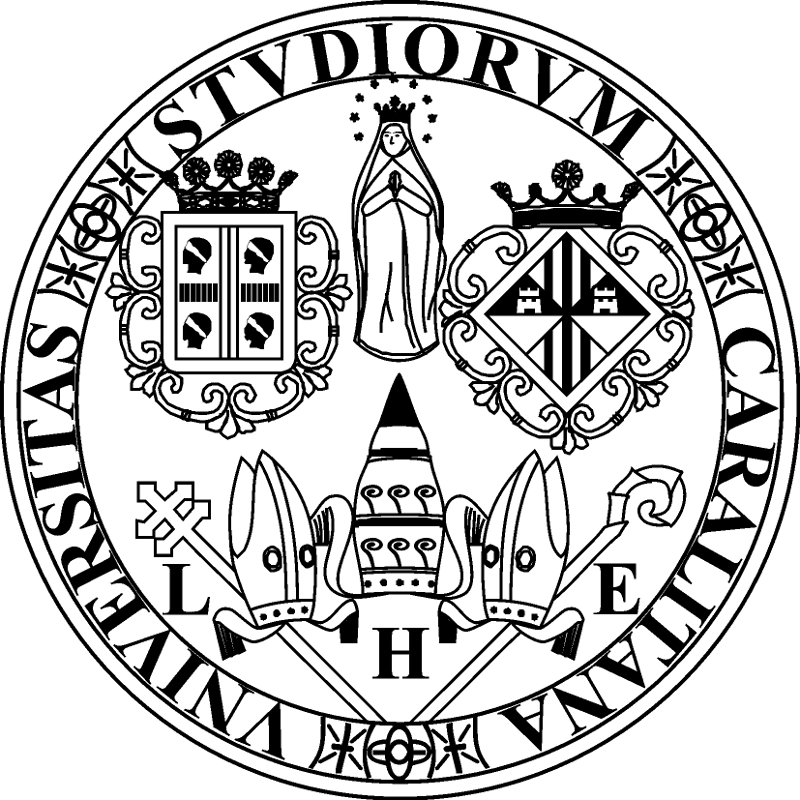
\includegraphics[width=0.3\textwidth]{images/logo.png}
\end{figure}
\begin{center}
    \textsc{ \LARGE{Università degli Studi di Cagliari \\}}
	\textsc{ \LARGE{Facoltà di Scienze\\ }}
	\textnormal{ \LARGE{Corso di Laurea Triennale in Informatica\\}}
	\vspace{30mm}
	\fontsize{10mm}{7mm}\selectfont 
    \textup{Synchronized P System Equivalence with Petri Nets with Inhibitor Arcs}\\
\end{center}

\vspace{25mm}

\begin{minipage}[t]{0.47\textwidth}
	\textnormal{\large{\bf Relatore:\\}}
	{\large Prof. Giovanni Michele Pinna}
\end{minipage}\hfill\begin{minipage}[t]{0.47\textwidth}\raggedleft
	\textnormal{\large{\bf Candidato:\\}}
	{\large Floris Alessandro\\ matr. 60/61/65913}
\end{minipage}

\vspace{20mm}

\centering{\large{Anno Accademico 23/24 \\ Cagliari - 25/09/24 }}

\end{titlepage}


\newpage 
\
\thispagestyle{empty}
\newpage

\tableofcontents
\thispagestyle{empty}

\newpage 
\
\thispagestyle{empty}
\newpage

\clearpage
\pagenumbering{arabic} 

\chapter{Introduction}

Membrane computing is a branch of natural computing, a field of research which tries to imitate nature in the ways it computes.
The obtained computing models are distributed parallel devices, called P systems (known also as Membrane systems).
The main aim of membrane computing is to model parallel systems inspired by the structure and behaviour of biological cells, but P systems are also rather powerful, equivalent with Turing machines.\\

Petri nets are an abstract, formal model of information flow.
The major use of Petri nets is to model concurrent systems, and P systems can be seen as highly concurrent systems, indeed in this thesis we try (successfully) to model the behaviour of a particular class of membrane systems, membrane systems which use synchronization among the rules of the same membrane, that we're gonna just call \textit{synchronization P systems}, using extended Petri nets with inhibitor arcs. \\

In the next chapter we we will elaborate and formally define what P systems, Petri nets and their extensions are.
In the third chapter we first establish a link between a basic class of P systems and Petri nets, then between synchronization P systems and Petri nets with inhibitor arcs.
Chapter 4 provides the proof that computations of a synchronized P systems coincide with step sequences of the relative extended Petri net. 
Finally, in chapter 5 we talk about future developments and changes to adopt.
\chapter{Background}

In this chapter we introduce some general notions as well as a more deep understanding of what P systems and Petri nets are.

\section{Basic Definitions}

\begin{definition}[Multiset]
Let $U$ be an arbitrary set. A multiset over U is a mapping \newline $m : U \rightarrow N$.
The multiplicity of an element $u$ in $m$ is given by the natural number $m(u)$.
\end{definition}

The operator $\oplus$ denotes multiset union: $m \oplus m' = m(u) + m'(u)$ for each $u$.

\begin{definition}[Alphabet]
An alphabet is a finite nonempty set of abstract symbols. Given an alphabet $V$, we denote by $V^*$
the sets of all finite strings of elements in $V$, including the empty string $\lambda$.
Every string $v \in V$ describes a multiset over $V$.
\end{definition}

\section{P Systems}

Membrane computing is a branch of natural computing, introduced by Gheorghe Paun with the definition of P systems in \cite{puaun2000computing,puaun2002membrane,paun1999computing}.

Membrane systems are based upon the notion of \textit{membrane structure}, which is a structure composed by several cell-membranes, hierarchically embedded in a main membrane called the \textit{skin membrane}.
The membranes delimit \textit{regions} and we associate with each region a set of \textit{objects}, described by some symbols over an alphabet, and a set of \textit{evolution rules}.
In the basic variant, the objects evolve according to the evolution rules, which can modify the objects to obtain new objects.
The evolution rules are applied in a maximally parallel manner: at each step, all the objects which can evolve should evolve.
If a computation \textit{halts}, so no further evolution rule can be applied, the result of the computation is defined to be the number of objects in a specified membrane.

\begin{definition}[P system]
A P system (of degree $d$, with $d \geq 1$) is a tuple
\[ \Pi = (V,\mu,w^0_1,...,w^0_d,R_1,...,R_d, i_0)\]
where:
\begin{enumerate}
  \item $V$ is an alphabet; its elements are called objects;
  \item $\mu$ is a membrane structure consisting of $d$ membranes (labeled with $1,2,...,d$);
  \item $w^0_1, 1 \leq i \leq d$, are strings from $V^*$ representing multisets over $V$ associated
  with the regions $1,2,...,d$ of $\mu$;
  \item $R_i, 1 \leq i \leq d$, are finite sets of evolution rules over $V$ associated 
  with the regions $1,2,...,d$ of $\mu$; these evolution rules are of the form $u \rightarrow v$,
  where $u$ and $v$ are strings from $V*$;
  \item $i_0$ is a number between 1 and $d$ which specifies the output membrane of %\Pi;
\end{enumerate}
A configuration of $\Pi$ is a tuple $C=(w_1,...,w_d)$ of multisets of objects, and 
$C_0=(w^0_1,...,w^0_d)$ is the initial configuration.
\end{definition}

According to \cite{agrigoroaiei2010flattening}, any P system can be flattened to a system of degree 1, we call this type of P systems \textit{flat P systems}.
For the sake of simplicity, from now on when we talk about P systems we refer to flat P systems.

\begin{definition}[Flat P system]
A flat P system is a P system of degree one
\[ \Pi = (V,\mu,w^0,R) \]

Given the fact that we're working with a one degree system we removed the subscript from $w$ and $R$. 
A configuration of $\Pi$ is a singleton $C=(w)=w$ of a multiset of objects, and 
$C_0=(w^0)=w^0$ is the initial configuration.
\end{definition}

The following example will clarify the definition of a P system.
\begin{example}
\label{ex:flat_membrane}
Consider the system of degree 1:
\begin{description}
   \item $\Pi=(V,\mu,w^0,R)$,
   \item $V=\{a,b,c\}$,
   \item $\mu=[_{1}]_{1}$,
   \item $C_0=w^0=a^2b$,
   \item $R=\{r_1:a \rightarrow b, r_2:a \rightarrow c\}$
\end{description}    
\end{example}

The system is represented in Fig 2.1.

\begin{figure}[h]
\centering

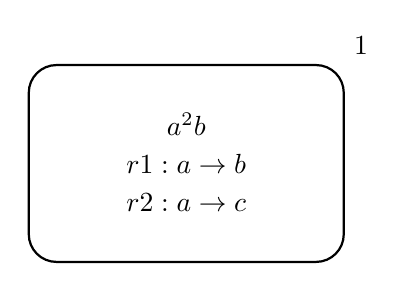
\begin{tikzpicture}
    \draw[thick, rounded corners=10pt] (0, 0) rectangle (4, 2.5) node[above right] {1};
    
    \node at (2, 1.75) {$a^2b$};
    \node at (2,1.25) (rule) {$r1: a \rightarrow b$};
    \node at (2,0.75) (rule) {$r2: a \rightarrow c$};
\end{tikzpicture}

\caption{}
\label{}
\end{figure}

The possibilities to evolve in one step from the initial configuration are: 
\begin{description}
    \item $C=w=b^3$, obtained applying $r=r_1^2$,
    \item $C=w=bc^2$, obtained applying $r=r_2^2$,
    \item $C=w=b^2c$, obtained applying $r=r_1 r_2$
\end{description}

\subsection{Synchronized P systems}

In this section we introduce a new class of P systems, P systems with \textit{synchronization among the rules of the same membrane}.
In the previous section we've seen a kind of synchronization where all regions use their rules in parallel in the maximal mode.
That synchronization that we're interested in is different, more exactly, a rule synchronizing with a non-empty set of rules is applicable at least once only if each rule from the set of rules is applicable at least once.

We call P systems with this kind of synchronization \textit{synchronized P systems}.
They are introduced and studied in \cite{aman2019synchronization,aman2022power}.

\begin{definition}[Synchronized P system]
A synchronized P system is a tuple

\[ \Pi = (V,\mu,w^0,R,\rho) \]

where:
\begin{enumerate}
    \item $(V,\mu,w^0,r)$ is a flat P system;    
    \item $\rho$ is a partial relation defined over the set $R$ of rules specifying
    the synchronization relation over the rules;
    $\rho$ is irreflexive, asymmetric and transitive;
\end{enumerate}
\end{definition}

% Questa parte è da cancellare e riscrivere 
Let's try to understand better what synchronization means:
let $(r1,r2) \in \rho$; if $r1$ is executed at least one time, then also
$r2$ has to be executed at least one time during this step, and vice versa; if that is not possible neither of them will be executed during the current step.

We use the following notation to describe an instance of $\rho$: 
$\rho=((r1 \otimes r2),(r3 \otimes r4 \otimes r5))$.
This means that $r_1$ can be executed only and only if $r_2$ can be executed at least one time;
in addition, $r_1$ it's executed at least one time only and only if also $r_2$ it's executed at least one time.

\begin{definition}[synchronization rule]
\label{def:sync_rule}
We define a synchronization rule $r_s$ as a set of rules.\\
For example $r_s=r_1 r_2 = r_1 \otimes r_2$ could be a synchronization rule.
\end{definition}

\begin{example}
    We modify \hyperref[ex:flat_membrane]{$example 1$} adding the synchronization 
    $r_1 \otimes r_2$.\\
    Now there is only one possible way to evolve in one step from the initial configuration:\\
    $C=w=b^2c$, obtained applying $r=r_1 r_2=r_1 \otimes r_2=r_{12}$;
\end{example}

In this previous example we have illustrated how the maximal parallelism behaviour is modified when synchronization of rules is used.

\section{Semantics of Synchronized P Systems}

For the purposes of this thesis, it is useful to decompose a synchronized P system computation step into multiple micro steps.
We know from \cite{busi2007causality} that the classical maximal parallelism semantics is equivalent to a causal semantics where a maximal parallelism evolution step is represented as a sequence of simple evolution steps, which are obtained by the application of a single evolution rule.

We need then to modify what a configuration is.
To represent the states of the system reached after the execution of a non maximal sequence of simple evolution rules, we introduce the notion of \textit{partial configuration} of a system.
In a partial configuration, the contents of each region is represented by two multisets.

\begin{definition}[partial configuration]
A partial configuration of $\Pi$ is a tuple $C_p=(w,w')$ 
where $w$ is the active multiset and $w'$ is the deposit (or frozen) multiset.
\end{definition}

A configuration is then a partial configuration containing no objects in the deposit;
So the initial configuration should be $C_0=(w,\emptyset)$.
Configurations represent the states reached after the execution of a maximal parallelism computation step.

Each micro step is obtained by the application of a single evolution rule.
When no evolution rule can be applied a special rule (function) will be used.

We introduce a new function, the \textit{transport function}, that transports the objects from the deposit multiset to the active multiset; this function will be used in the definition of the maximal parallelism computation step.

\begin{definition}[transport function]
Let $C=(w,w')$ be a partial configuration of $\Pi$.\newline
The transport function $\delta: Conf_\Pi \rightarrow Conf_\Pi$ is defined as follows:\newline
$\delta((w,w'))=(w \oplus w', \emptyset)$
\end{definition}

Using the classical maximal parallelism semantics a rule $r$ that is part of a synchronization rule $r_s$ can be executed during a computational step only if $r_s$ is executed in the same computational step.
In our causal semantics we decompose a computational step in micro steps; it results that $r$ can be executed only if $r_s$ has been executed in a previous micro step that is part of the same computational step.
Now we describe how our semantics works with the following inference rules:\newline

\noindent
\begin{tabular}{ @{} r c l @{} }
  R1. & \infer{(w,w') \xrightarrow{\delta} (w \oplus w', \emptyset) }
{\text{no rule is applicable}} \\ \\
  R2. & \infer{(w,w') \xrightarrow{r_s} (w - lhs(r_s), w' + rhs(r_s)) }
{\text{$r_s$ is enabled in $(w,w')$}} \\ \\
  R3. & \infer{(w,w') \xrightarrow{r} (w - lhs(r_s), w' + rhs(r_s)) }
{\text{$r$ is enabled in $(w,w')$ and if $r$ is part of $r_s$, $r_s$ has been executed}} \\ \\
\end{tabular}

\begin{definition}[computational step of causality semantics]
In our causality semantics a computational step is a ordered sequence of micro step, where each micro step is obtained by the application of a single evolution rule: 
$r_1, ..., r_k$ where $r_i \in R$ or $r_i \in R_s$ for $i=1,...,k$
\end{definition}

Let's see an example of our new semantics.
\begin{example}
    Consider the system 
    \[ \Pi = (\{a,b,c,d\},[_1]_1,a^2bc,\{r_1:a \rightarrow b, r_2: b \rightarrow c\}, \{r_{s1}: r_1 r_2\}) \]
    The only rule we can apply is R2, since $r_{s1}$ is enabled in $(a^2bc,\emptyset)$ and no other evolution rule is.
    After this micro step we have $C_p = (ac,bc)$.
    Now we can apply rule R3, so we apply the evolution rule $r_1$ thus obtaining the partial configuration $C_p = (c,b^2c)$.
    No other evolution rule is enabled, so R1 is the only rule applicable, and we get 
    $C = (b^2c^2)$, and this is the configuration obtained after a whole computational step.
\end{example}

\section{Petri Net}

Here we define in a formal way what a Petri Net is.

\subsection{Petri Nets with Inhibitor Arcs}

Here we extend the latter definition of a Petri Net with the concept of inhibitor arcs.

\chapter{A New Semantics for Synchronized P Systems}

For the purpose of this thesis it is useful to define a new semantics for our synchronized P systems.
We know that a rule $r$ that compose a synchronization rule $r_s$ can be executed if and only $r_s$ it's executed during the same evolution step. 
So we could say that the application of the rule $r$ causally depends on the application of the synchronization rule $r_s$.\newline

Let's say that an evolution step is an ordered sequence of micro evolution steps obtained by the application of a single evolution rule.
So now a classical maximal parallelism evolution step is represented as a sequence of simple evolution steps.
This is called \textit{causal semantics}, and was first defined for a basic P system in \cite{busi2007causality}.

\begin{definition}[Configuration and partial configuration]
    In our new semantics a configuration is a pair $C=(w_1,w_2)$ where $w_1$ is the active multiset and $w_2$ is the deposit (or frozen) multiset.\newline
    We call a configuration $C=(w_1,w_2)$ where $w_2 \neq \emptyset$ a \textit{partial configuration}; if $w_2 = \emptyset$ we'll refer to $C$ as a configuration.
\end{definition}

So now the initial configuration of a P system $\Pi$ is $C_0=(w_1,\emptyset)$.
Doing a whole evolution step means to go from a configuration $(w_1,\emptyset)$ to another configuration $(w_1',\emptyset)$ passing through a sequence of micro steps.

Before providing a new definitions of an evolution step and a micro step, we need a some auxiliary definitions.
We first introduce the concept of \textit{causal configuration}, then we introduce a new function, the \textit{transport function}, that transports the objects in the deposit multiset to the active multiset; it can be seen as a special evolution rule proper of the semantics itself.

\begin{definition}[Causal configuration]
    A causal configuration is a tuple 
    \[CC = \langle C, \Gamma \rangle\]
    where $C$ is a configuration (or a partial configuration) and $\Gamma$ is a set of synchronization rules.
    Given an initial configuration $C_0$ the respective causal configuration is $CC = \langle C_0,\emptyset\rangle$.
\end{definition}

\begin{definition}[transport function]
    Let $C=(w,w')$ be a partial configuration of $\Pi$.\newline
    The transport function $\delta: Conf_\Pi \rightarrow Conf_\Pi$ is defined as follows:\newline
    $\delta((w,w'))=(w \oplus w', \emptyset)$
\end{definition}

With the notion of transport function and causal configuration we can now define what a computational step and a micro step are.

\begin{definition}[computational step and micro steps]
    A computational step is defined as an ordered sequence of micro steps.\newline
    $(w_1,\emptyset) \Rightarrow (w_1',\emptyset)$ is a computational step if and only if 
    there exists $k$ micro steps such that $(w_1,\emptyset) \xrightarrow{r_1} (w_1'',w_2'')
    \xrightarrow{r_2} \cdots \xrightarrow{r_k} (w_1',\emptyset)$ where $r_k$ is the transport function $\delta$.
    We also define $r=<r_1,\ldots,r_k>$ as the ordered sequence of evolution rules applied at each micro step.
\end{definition}

Now we describe how our semantics works with the following inference rules:\newline

\noindent
\begin{tabular}{ @{} r c l @{} }
  R1. & \infer{
  \langle(w,w'),\Gamma\rangle \xrightarrow{\delta} \langle(w \oplus w', \emptyset),\emptyset\rangle
  }
{\text{no rule is enabled}} \\ \\
  R2. & \infer{
  \langle(w,w'),\Gamma\rangle \xrightarrow{r_s} \langle(w - lhs(r_s), w' + rhs(r_s)),\Gamma \cup 
  \{r_s\} \rangle 
  }
{\text{$r_s$ is enabled in $(w,w')$}} \\ \\
  R3. & \infer{
  \langle (w,w'), \Gamma \rangle \xrightarrow{r} \langle (w - lhs(r_s), w' + rhs(r_s)), \Gamma \rangle 
  }
{\text{$r$ is enabled in $(w,w')$ and if $r$ compose $r_s$, $r_s \in \Gamma$}} \\ \\
\end{tabular}

Let's see an example of our new semantics.
\begin{example}
    Consider the system 
    \[ \Pi = (\{a,b,c,d\},[_1]_1,a^2bc,\{r_1:a \rightarrow b, r_2: b \rightarrow c\}, \{r_{12}: r_1 r_2\}) \]
    The only rule we can apply is R2, since $r_{12}$ is enabled in $(a^2bc,\emptyset)$ and no other evolution rule is.
    After this micro step we have $C = (ac,bc)$.
    Now we can apply rule R3, so we apply the evolution rule $r_1$ thus obtaining the partial configuration $C = (c,b^2c)$.
    No other evolution rule is enabled, so R1 is the only rule applicable, and we get 
    $C = (b^2c^2)$, and this is the configuration obtained after a whole evolution step.
\end{example}
\chapter{Proof of Equivalence}

We now want to prove that a computational step of $\Pi$ is equivalent to a computational step of $PTI_\Pi$.
So we know from chapter 2 that a $\Pi$ step is an ordered sequence of micro steps.
Each micro step is the application of a single evolution rule;
We have thus to prove that a micro step of $\Pi$ is equivalent to a step of our Petri net.
The following is an example of a micro step: $(w_1,w_2) \xrightarrow{r} (w_1',w_2')$.
Let's map the execution of a rule to the execution of a multiset of transitions.

\begin{definition}[mapping micro steps]
    Given a micro step $(w_1,w_2) \xrightarrow{r} (w_1',w_2')$ from $\Pi$:
    \begin{enumerate}
        \item if $r=r_s$ then $t^s$ is executed;
        \item if $r=r$ then $t^r$ is executed, and if during the precedent step a transition $t^s$ has been executed, then also fire $t^s'$;
        \item if $r=\delta$ then $\gamma$ is executed;
    \end{enumerate}
\end{definition}

Since a configuration $C$ in $\Pi$ is a pair $C=(w1,w2)$ we need to change \hyperref[def:map_conf]{$3.1.1$}.

\begin{definition}[$\psi$ operator]
We define a function $\psi: M \rightarrow M$ that takes a multiset M and returns a subset of it 
that contains only the places $p=(a)$.
\end{definition}

\begin{fact}[]
$v(C_0)=\psi(M_{0})$
\end{fact}

\chapter{Conclusions and Future Developments}
\chapter{Conclusions and Future Developments}
\printbibliography[heading=bibintoc, title={References}]
\addcontentsline{toc}{chapter}{Acknowledgments}
\chapter*{Acknowledgments}
Grazie a tutti.

\end{document}